% !TeX root = ../../../Main.tex
\chapter{Trajectory Optimization with Policy Iteration}
\label{chapter5}
\section{2D Environment}

In the context of this work, the aircraft is treated as a mass point. Rotational dynamics are neglected. This is sufficient for trajectory optimization algorithms. See \cite{Fichter2009} for more details. 


In this scenario, the glider moves in the geodetic vertical plane. Its control is the angle of attack $\alpha$. When $\alpha$ is increased, the lift $L$ increases. This results in an increase of $\gamma$, as can be seen in equation \ref{eq:dotgamma}. This way the agent can control its velocity vector and therefore its position. All other parameters of the glider are shown in appendix \ref{appendix_A}. Any 3D-Scenario where the horizontal trajectory is restricted by obstacles or the optimal ground trace is obvious can be regarded as a 2D problem. The only control variable to be optimized is then the angle of attack or an equivalent quantity (e.g. vertical acceleration).

\subsection{Policy Representation}

As the Policy Iteration algorithm is running on a rectangular grid and the states that are updated do not change, a table that stores the greedy action for every state is sufficient for the Policy Iteration algorithm. Once the optimal policy is found, a neural network is trained to approximate the optimal action for each of the states on the grid. This policy is then used to do TRPO.

\subsection{Equations of Motion}

The physical state of the glider in the geodetic vertical plane consists of the position $\boldsymbol{{}_g r}=[x,z]^T$ and velocity $\boldsymbol{{}_g v}=[{}_g u_K,{}_g w_K]^T$. Apart from the geodetic reference frame (index g), a body fixed frame (index f), a trajectory fixed frame (index k) and an aerodynamic frame (index a) are used to describe the glider dynamics. In the vertical plane, coordinates can be transformed between the frames by a rotation around the y-axis. Figure \ref{fig:coords2d} illustrates the transformation angles that connect the reference frames. 

In the vertical plane, there are 4 state variables, $x$, $z$, $u=\dot{x}$ and $w=\dot{z}$, each with respect to a geodetic reference frame that has its origin at a point on the earth surface. The aerodynamic forces are often expressed in an aerodynamic reference frame. The coordinate transformations $u$ and $w$ can also be expressed by $V$ and $\phi_K$.

The dynamics in the vertical plane are given by the following equations. They are taken from \cite{Fichter2009}. 

\begin{equation}
\dot{x} = V \; cos\phi_K
\end{equation}

\begin{equation}
\dot{z} = - V \; sin\phi_K
\end{equation}

\begin{equation}
\dot{V} = -\frac{D + g \; cos\phi_K}{m}
\end{equation}

\begin{equation}
\dot{\phi_K} = \frac{L}{V \; m} - \frac{g \; cos{\phi_K}}{V} 
\label{eq:dotgamma}
\end{equation}

where $L = q \; c_L \; S$, $D = q \; c_D \; S = \frac{\rho}{2} \; V^2 \; c_d \; S$ and $V=\sqrt{u^2+w^2}$.

\subsection{Discretization of the State- and Action Space}
\label{sec:disc2d}
The state space is discretized with a rectangular grid, i.e. it is replaced by a set of points $s_n=[x_k,z_l,u_m,w_n]$ evenly distributed across all dimensions.

\begin{figure}
	\centering
	\tikzsetnextfilename{stategrid}
	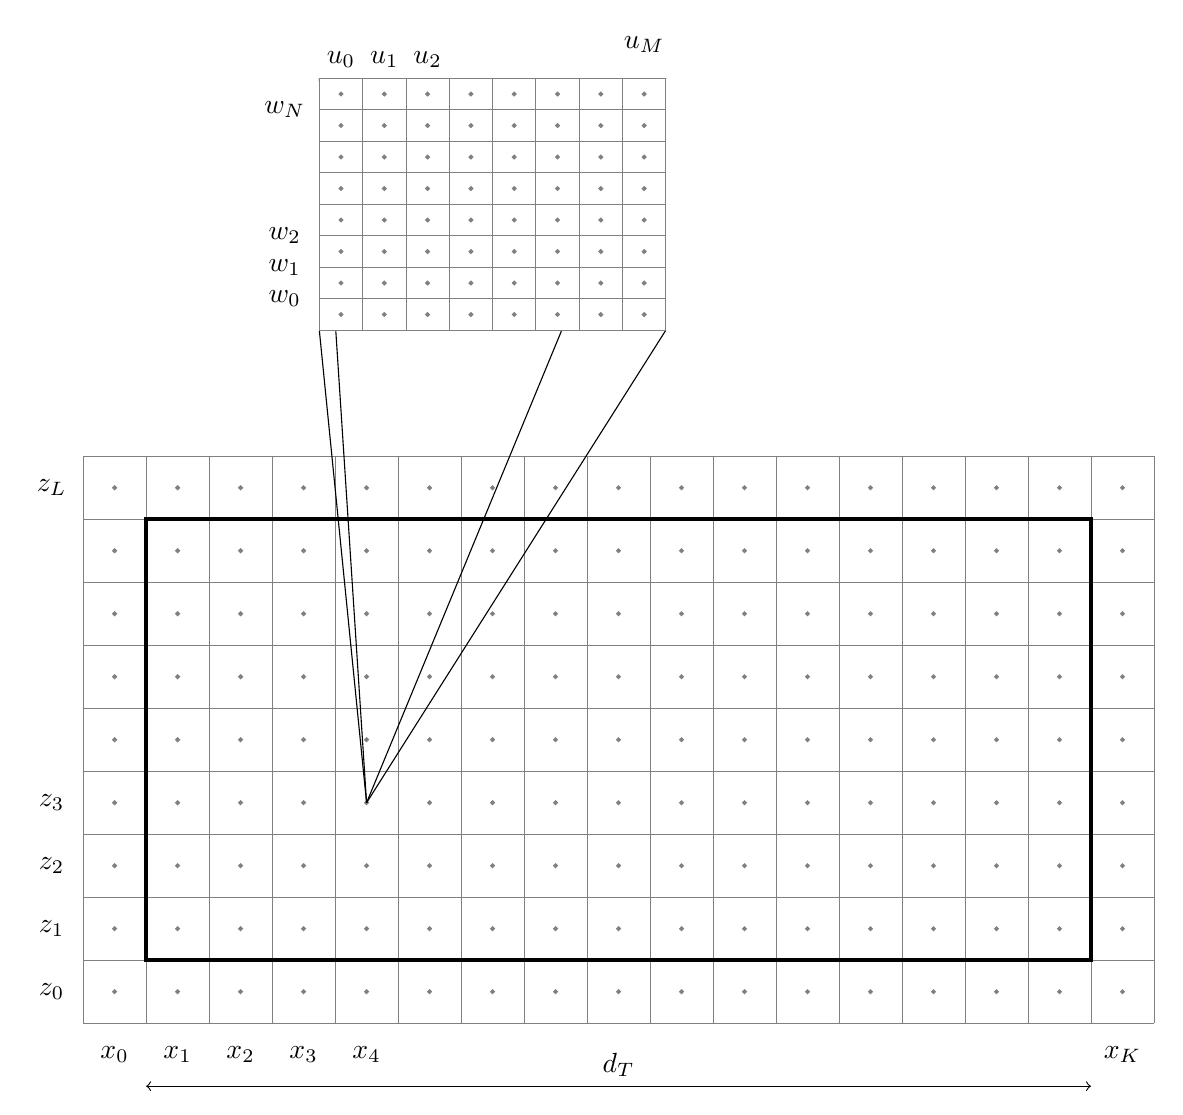
\begin{tikzpicture}[scale=0.8]
		\foreach \col in {-1,0,1,2,3,4,5,6,7,8,9,10,11,12,13,14,15,16}{
			\draw[color=gray, line width=0.3pt] (\col,-1) -- +(0,9);
		}
		\foreach \row in {-1,0,1,2,3,4,5,6,7,8}{
			\draw[color=gray, line width=0.3pt] (-1,\row) -- +(17,0);
		}
		\draw[draw=black, line width=1.5pt] (0,0) rectangle (15,7);
		\foreach \x in{-0.5,0.5,1.5,2.5,3.5,4.5,5.5,6.5,7.5,8.5,9.5,10.5,11.5,12.5,13.5,14.5,15.5}{
			\foreach \z in {-0.5,0.5,1.5,2.5,3.5,4.5,5.5,6.5,7.5}{
				\draw[draw=gray, fill=gray] (\x,\z) circle (0.03cm);
			}
		}

		\foreach \i in {0,1,2,3,4}{
			\node at (\i-0.5,-1.5) {$x_\i$};
		}
		\node at (15.5,-1.5) {$x_K$};
		\foreach \j in {0,1,2,3}{
			\node at (-1.5,\j-0.5) {$z_\j$};
		}
		\node at (-1.5,7.5) {$z_L$};
		\draw (3.5,2.5) -- (2.75,10);
		\draw (3.5,2.5) -- (8.25,10);
		\draw (3.5,2.5) -- (2.75,14);
		\draw (3.5,2.5) -- (8.25,14);
		\draw [color=gray, fill=white] (2.75,10) rectangle (8.25,14);
		\foreach \vcol in {1,2,3,4,5,6,7}{
			\draw[color=gray, line width=0.3pt] (2.75+\vcol*0.6875,10) -- +(0,4);
		}
		\foreach \vrow in {1,2,3,4,5,6,7}{
			\draw[color=gray, line width=0.3pt] (2.75,10+\vrow*0.5) -- +(8*0.6875,0);
		}
		\foreach \u in {-3.5,-2.5,-1.5,-0.5,0.5,1.5,2.5,3.5}{
			\foreach \w in {-3.5,-2.5,-1.5,-0.5,0.5,1.5,2.5,3.5}{
				\draw[draw=gray, fill=gray] (5.5+\u*0.6875,12+\w*0.5) circle (0.03cm);
			}
		}
		\foreach \k in {0,1,2}{
			\node at (3.09375+\k*0.6875,14.3) {$u_\k$};
		}
		\node at (3.09375+7*0.6875,14.53) {$u_M$};
		\foreach \l in {0,1,2}{
			\node at (2.2,10.5+\l*0.5) {$w_\l$};
		}
		\node at (2.2,13.5) {$w_N$};
		\draw[<->] (0,-2) -- node[above] {$d_T$} (15,-2);
%		\node at (3.5,2.5) {Text} ;
	\end{tikzpicture}
	\caption{The discretized state space in all 2d scenarios. For $x_4$ and $z_3$, the grid for the speed vector is drawn.}
	\label{tikz:2d_state_space_discretized}
\end{figure}

In the 2D-scenario, the action space is one-dimensional, with the only action being the angle of attack $\alpha$. For the policy improvement step, a finite number of evenly spaced actions is sampled from the infinite set of possible actions between $\alpha_{min} = 0$ and $\alpha_{max}=0.2$. Assuming that the mapping from actions to returns is continuous, the action that yields the maximum expected return out of the sampled actions is an approximation of the true greedy action.

By discretization, the continuous trajectory optimization problem is made time- and space-discrete. For the purpose of keeping calculation time low, a sample time $\Delta t$ of $1s$ is used for the 1000m and 2000m flights. With a speed of $15-25 \frac{\text{m}}{\text{s}}$, the agent covers about $15-25\text{m}$ within one time step. In the scenarios, where the agent has to cover 500m, the sample-time is $0.5s$. The grid points should be separated by approximately that distance in order to make tabular solution methods feasible. For the different scenarios, this yields the grid resolutions shown in table \ref{tab:grids}.
\begin{table}
	\begin{center}
		\begin{tabular}{r|c c c}
			distance & $500m$ & $1000m$ & $2000m$ \\ \hline
			$n_x$ & 52 & 52 & 102 \\
			$n_z$ & 42 & 22 & 22\\
			$n_u$ & 8 & 8 & 8 \\
			$n_w$ & 8 & 8 & 8
		\end{tabular}
	\end{center}
	\caption{Grid parameters for trajectory optimization}
	\label{tab:grids}
\end{table}

\section{3D Environment}

todo

\subsection{Discretization of the state and action space}
\label{sec:disc3d}
todo